\subsection{SGX Memory Access Protection}
\label{sec:sgx_access_protection}

SGX guarantees that the software inside an enclave is isolated from all the
software outside the enclave, including the software running in other enclaves.
This isolation guarantee is at the core of SGX's security model.

It is tempting to assume that the main protection mechanism in SGX is the
Memory Encryption Engine (MEE) described in
\S~\ref{sec:sgx_uncore_modifications}, as it encrypts and MACs the DRAM's
contents. However, the MEE sits in the processor's memory controller, which is
at the edge of the on-chip memory hierarchy, below the
caches~(\S~\ref{sec:caching}). Therefore, the MEE cannot protect an enclave's
memory from software attacks.

% Page-Based Access Control: SDM S 38.5
% Interactions with Paging: SDM S 42.4
% ISCA SGX Slide 27

The root of SGX's protections against software attacks is a series of memory
access checks which prevents the currently running software from accessing
memory that does not belong to it. Specifically, non-enclave software is only
allowed to access memory outside the PRM range, while the code inside an
enclave is allowed to access non-PRM memory, and the EPC pages owned by the
enclave.

% SGX relies on PMH to prevent unauthorized access to EPC pages
%   US 8,972,746 B2 - 31:1-10

Although it is believed~\cite{evtyushkin2014isox} that SGX's access checks are
performed on every memory access check, Intel's patents disclose that the
checks are performed in the Page Miss Handler~(PMH,~\S~\ref{sec:tlbs}), which
only handles TLB misses.


\subsubsection{Functional Description}
\label{sec:sgx_access_concepts}

The intuition behind SGX's memory access protections can be built by
considering what it would take to implement the same protections in a trusted
operating system or hypervisor, solely by using the page tables that direct the
CPU's address translation feature~(\S~\ref{sec:paging}).

The hypothetical trusted software proposed above can implement enclave
entry~(\S~\ref{sec:sgx_eenter}) as a system call~\S~\ref{sec:syscalls} that
creates page table entries mapping the enclave's memory. Enclave
exit~(\S~\ref{sec:sgx_eexit}) can be a symmetric system call that removes the
page table entries created during enclave entry.  When modifying the page
tables, the system software has to consider TLB coherence
issues~(\S~\ref{sec:tlbs}) and perform TLB shootdowns when appropriate.

SGX leaves page table management under the system software's control, but it
cannot trust the software to set up the page tables in any particular way.
Therefore, the hypothetical design described above cannot be used by SGX as-is.
Instead, at a conceptual level, the SGX implementation approximates the effect
of having the page tables set up correctly by inspecting every address
translation that comes out of the Page Miss Handler~(PMH,~\S~\ref{sec:tlbs}).
The address translations that do not obey SGX's access control restrictions
are rejected before they reach the TLBs.

SGX's approach relies on the fact that software always references memory using
virtual addresses, so all the micro-ops~(\S~\ref{sec:out_of_order}) that reach
the memory execution units~(\S~\ref{sec:execution_units}) use virtual addresses
that must be resolved using the TLBs before the actual memory accesses are
carried out. By contrast, the processor's microcode~(\S~\ref{sec:microcode})
has the ability to issue physical memory accesses, which bypass the TLBs.
Conveniently, SGX instructions are implemented in microcode
(\S~\ref{sec:sgx_microcode_modifications}), so they can bypass the TLBs and
access memory that is off limits to software, such as the EPC page holding an
enclave's SECS\~(\S~\ref{sec:sgx_secs}).

% Enclave Page Cache Map (EPCM): SDM S 37.5.1, SDM S 38.19
% Security Information (SECINFO): SDM S 38.11, S 38.11.{1,2}
% SECINFO.FLAGS: SDM S 38.11.1
% PAGE_TYPE Field Definition: SDM S 38.11.2

The SGX address translation checks use the information in the Enclave Page
Cache Map~(EPCM,~\S~\ref{sec:sgx_epcm}), which is effectively an inverted page
table that covers the entire EPC. This means that each EPC page is accounted
for by an EPCM entry, using the structure is summarized in
Table~\ref{fig:sgx_epcm_entry}. The EPCM fields were described in detail in
\S~\ref{sec:sgx_epcm}, \S~\ref{sec:sgx_paging}, \S~\ref{sec:sgx_tcs},
\S~\ref{sec:sgx_eblock}, and \S~\ref{sec:sgx_va}.

% EPCM contains SECS_SID (the SID for the owning SECS) for each EPC page
%   US 8,972,746 B2 - 29:26-33
% EPCM Flags
%   US 8,972,746 B2 - Tables 4-16 and 4-17, column 20

\begin{table}[hbt]
  \centering
  \begin{tabularx}{\columnwidth}{| l | r | X |}
  \hline
  \textbf{Field} & \textbf{Bits} & \textbf{Description}\\
  \hline
  VALID & 1 & 0 for un-allocated EPC pages \\
  \hline
  BLOCKED & 1 & page is being evicted \\
  \hline
  R & 1 & enclave code can read \\
  \hline
  W & 1 & enclave code can write \\
  \hline
  X & 1 & enclave code can execute \\
  \hline
  PT & 8 & page type (Table~\ref{fig:sgx_pt_values}) \\
  \hline
  ADDRESS & 48 & the virtual address used to access this page \\
  \hline
  ENCLAVESECS &  & the EPC slot number for the SECS of the enclave owning the
                     page \\
  \hline
  \end{tabularx}
  \caption{
    The fields in an EPCM entry.
  }
  \label{fig:sgx_epcm_entry}
\end{table}

\begin{table}[hbt]
  \centering
  \begin{tabularx}{\columnwidth}{| l | l | X |}
  \hline
  \textbf{Type} & \textbf{Allocated by} & \textbf{Contents}\\
  \hline
  PT\_REG & \texttt{EADD} & enclave code and data \\
  \hline
  PT\_SECS & \texttt{ECREATE} & SECS (\S~\ref{sec:sgx_secs}) \\
  \hline
  PT\_TCS & \texttt{EADD} & TCS (\S~\ref{sec:sgx_tcs}) \\
  \hline
  PT\_VA & \texttt{EPA} & VA (\S~\ref{sec:sgx_va}) \\
  \hline
  \end{tabularx}
  \caption{Values of the PT (page type) field in an EPCM entry.}
  \label{fig:sgx_pt_values}
\end{table}

% Intel SGX Interaction with Protection Keys: SDM S 42.18
%   Enclave checks occur after protection keys checks
% ISCA 2015 SGX: Slide 27

Conceptually, SGX adds the access control logic illustrated in
Figure~\ref{fig:sgx_tlb_miss_checks} to the PMH. SGX's security checks are
performed after the page table attributes-based
checks~(\S~\ref{sec:page_table_attributes}) defined by the Intel architecture.
It follows that SGX's access control logic has access to the physical address
produced by the page walker FSM.

\begin{figure}[hbtp]
  \centering
  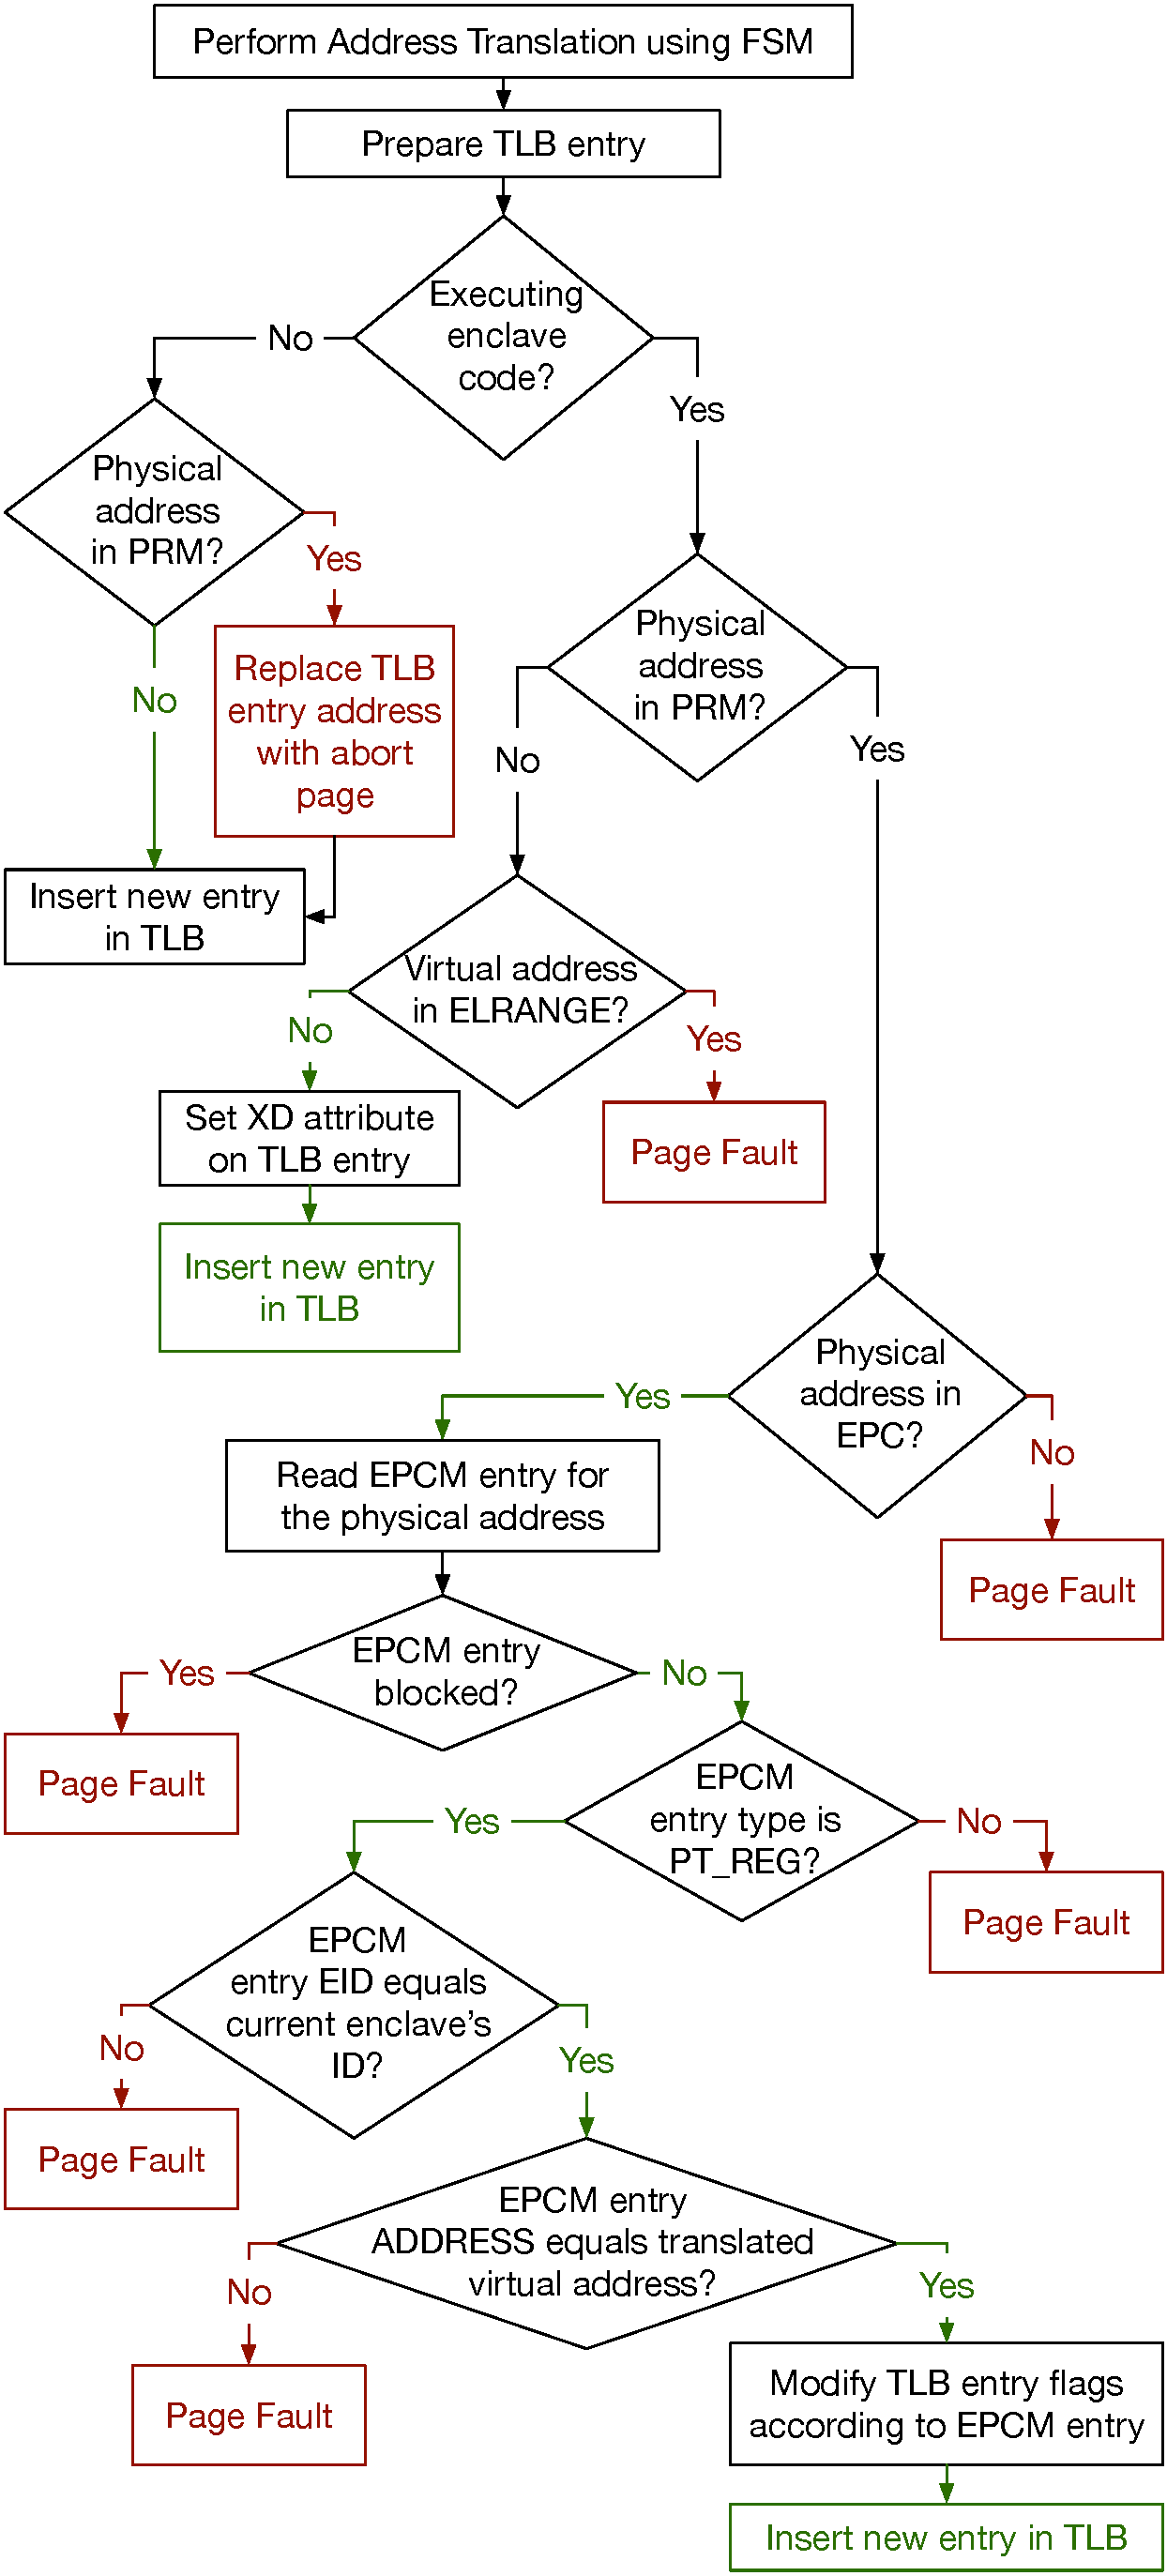
\includegraphics[width=85mm]{figures/sgx_tlb_miss_checks.pdf}
  \caption{
    SGX adds a few security checks to the PMH. The checks ensure that all the
    TLB entries created by the address translation unit meet SGX's memory
    access restrictions.
  }
  \label{fig:sgx_tlb_miss_checks}
\end{figure}

% EPC accessible only inside microcode extension mode or enclave mode
%   US 8,972,746 B2 - 8:26-29, 8:31-34
% EPC can only be accessed using linear addresses in enclave range
%   US 8,972,746 B2 - 8:29-31
% ECREATE defines linear access range, all addresses in range are protected
%   US 8,972,746 B2 - 31:12-25
% Linear addresses in enclave range that do not resolve to EPC are bounced
%   US 8,972,746 B2 - 8:35-40
% Enclave accesses to EPC pages are validated using EPCM valid bit
%   US 8,972,746 B2 - 8:41-45
% EPC page ownership is verified by looking at the page's SECS
%   US 8,972,746 B2 - 8:45-49
% EPC accesses check the linear address in the EPCM, prevent attacks
%   US 8,972,746 B2 - 8:50-62

SGX's security checks depend on whether the logical
processor~(\S~\ref{sec:cpu_core}) is in enclave mode~(\S~\ref{sec:sgx_threads})
or not. While the processor is outside enclave mode, the PMH allows any address
translation that does not target the PRM range~(\S~\ref{sec:sgx_prm}). When the
processor is inside enclave mode, the PMH performs the checks described below,
which provide the security guarantees described in \S~\ref{sec:sgx_paging}.

First, virtual addresses inside the enclave's virtual memory
range~(ELRANGE,~\S~\ref{sec:sgx_elrange}) must always translate into physical
addresses inside the EPC. This way, an enclave is assured that all the code and
data stored in ELRANGE receives SGX's privacy, integrity, and freshness
guarantees. Since the memory outside ELRANGE does not enjoy these guarantees,
the SGX design disallows having enclave code outside ELRANGE. This is most
likely accomplished by setting the disable
execution~(XD,~\S~\ref{sec:page_table_attributes}) attribute on the TLB entry.

Second, an EPC page must only be accessed by the code of the enclave who owns
the page. For the purpose of this check, each enclave is identified by the
index of the EPC page that stores the enclave's SECS~(\S~\ref{sec:sgx_secs}).
The current enclave's identifier is stored in the CR\_ACTIVE\_SECS microcode
register during enclave entry. This register is compared against the enclave
identifier stored in the EPCM entry corresponding to the EPC page targeted by
the address translation.

% EPC pages are identified by 0-based slot numbers
% SID = (page_phys_addr - epc_base_phys_addr) >> 2
%   US 8,972,746 B2 - 29:5-23
% EPCM contains SECS_SID (the SID for the owning SECS) for each EPC page
%   US 8,972,746 B2 - 29:26-33

Third, some EPC pages cannot be accessed by software. Pages that hold SGX
internal structures, such as a SECS, a TCS~(\S~\ref{sec:sgx_tcs}), or a
VA~(\S~\ref{sec:sgx_va}) must only be accessed by SGX's microcode, which uses
physical addresses and bypasses the address translation unit, including the
PMH. Therefore, the PMH rejects address translations targeting these pages.

Blocked~(\S~\ref{sec:sgx_eblock}) EPC pages are in the process of being
evicted~(\S~\ref{sec:sgx_epc_eviction}), so the PMH must not create new TLB
entries targeting them.

Next, an enclave's EPC pages must always be accessed using the virtual
addresses associated with them when they were allocated to the enclave. Regular
EPC pages, which can be accessed by software, are allocated to enclaves using
the \texttt{EADD}~(\S~\ref{sec:sgx_eadd}) instruction, which reads in the
page's address in the enclave's virtual address space. This address is stored
in the LINADDR field in the corresponding EPCM entry. Therefore, all the PMH
has to do is to ensure that LINADDR in the address translation's target EPCM
entry equals the virtual address that caused the TLB miss which invoked the
PMH.

At this point, the PMH's security checks have completed, and the address
translation result will definitely be added to the TLB. Before that happens,
however, the SGX extensions to the PMH apply the access restrictions in the
EPCM entry for the page to the address translation result. While the public SGX
documentation we found did not describe this process, there is a
straightforward implementation that fulfills SGX's security requirements.
Specifically, the TLB entry bits P, W, and XD can be AND-ed with the EPCM entry
bits R, W, and X.


\subsubsection{EPCM Entry Representation}
\label{sec:sgx_epcm_format}

% EPC and EPCM
%   US 8,972,746 B2 - 4:36-58
% EPC pages are identified by 0-based slot numbers
% SID = (page_phys_addr - epc_base_phys_addr) >> 2
%   US 8,972,746 B2 - 29:5-23
% EPCM contains SECS_SID (the SID for the owning SECS) for each EPC page
%   US 8,972,746 B2 - 29:26-33
% Intel SGX Resource Enumeration Leaves: SDM S 37.7.2

Most EPCM entry fields have obvious representations. The exception is the
LINADDR and ENCLAVESECS fields, described below. These representations explain
SGX's seemingly arbitrary limit on the size of an enclave's virtual address
range (ELRANGE).

The SGX patents disclose that the LINADDR field in an EPCM entry stores the
virtual page number~(VPN,~\S~\ref{sec:paging_vpn}) of the corresponding EPC
page's expected virtual address, relative to the ELRANGE base of the enclave
that owns the page.

The representation described above reduces the number of bits needed to store
LINADDR, assuming that the maximum ELRANGE size is significantly smaller than
the virtual address size supported by the CPU. This desire to save EPCM entry
bits is the most likely motivation for specifying a processor model-specific
ELRANGE size, which is reported by the \texttt{CPUID} instruction.

The SDM states that the ENCLAVESECS field of an ECPM entry corresponding to an
EPC page indicates the SECS of belonging to the enclave that owns the page.
Intel's patents reveal that the SECS address in ENCLAVESECS is represented as
a physical page number~(PPN,~\S~\ref{sec:paging_ppn}) relative to the start of
the EPC. Effectively, this relative PPN is the 0-based EPC page index.

% ISCA 2015 SGX: Slide 196

The EPC page index representation saves bits in the ECPM entry, assuming that
the EPCM size is significantly smaller than the physical address space
supported by the CPU. The ISCA 2015 SGX tutorial slides mention an EPC size of
96MB, which is significantly smaller than the physical addressable space on
today's typical processors, which is $2^{36}$ - $2^{40}$ bytes.


\subsubsection{PMH Hardware Modifications}
\label{sec:sgx_pmh_hardware}

% SERR register implemented in PMH
%   US 8,972,746 B2 - 5:59-61
% PMH protects the enclave memory area via a range register.
%   US 8,972,746 B2 - 31:1-10, 31:31-36, 31:41-46, 31:65-67, 32:1-9
% Outside enclave mode, PMH protects access to EPC using a range register
%   US 8,972,746 B2 - 31:31-36
% Minimal PMH support for enclaves is MTRR to protect CMA access.
%   US 8,972,746 B2 - 31:65-67, 32:1-9
%   US 8,972,746 B2 - Table 8-1, column 31
% Better PMH support includes a linear access check to protect ELRANGE.
%   US 8,972,746 B2 - Table 8-1, column 31

The SDM describes the memory access checks performed after SGX is enabled, but
does not provide any insight into their implementation. Intel's patents hint at
three possible implementations that make different cost-performance tradeoffs.
This section summarizes the three approaches and argues in favor of the
implementation that requires the fewest hardware modifications to the PMH.

All implementations of SGX's security checks entail adding a pair of memory
type range registers~(MTRRs,~\S~\ref{sec:cacheability_config}) to the PMH.
These registers are named the \textit{Secure Enclave Range Registers}~(SERR)
in Intel's patents.  Enabling SGX on a logical processor initializes the SERR
to the values of the Protected Memory Range
Registers~(PMRR,~\S~\ref{sec:sgx_prm}).

Furthermore, all implementations have the same behavior when a logical
processor is outside enclave mode. The memory type range described by the SERR
is enabled, causing a microcode assist to trigger for every address translation
that resolves inside the PRM. SGX's implementation uses the microcode assist to
replace the address translation result with an address that causes memory
access transactions to be aborted.

The three implementations differ in their behavior when the processor enters
enclave mode~(\S~\ref{sec:sgx_threads}) and starts executing enclave code.

The alternative that requires the least amount of hardware changes sets up the
PMH to trigger a microcode assist for every address translation. This can be
done by setting the SERR to cover all the physical memory (e.g., by setting
both the base and the mask to zero). In this approach, the microcode assist
implements all the enclave mode security checks illustrated in
Figure~\ref{fig:sgx_tlb_miss_checks}.

A speedier alternative adds a pair of registers to the PMH that represents the
current enclave's ELRANGE and modifies the PMH so that, in addition to checking
physical addresses against the SERR, it also checks the virtual addresses
going into address translations against ELRANGE. When either check is true, the
PMH invokes the microcode assist used by SGX to implement its memory access
checks. Assuming the ELRANGE registers use the same base / mask representation
as variable MTRRs, enclave exists can clear ELRANGE by zeroing both the base
and the mask. This approach uses the same microcode assist implementation,
minus the ELRANGE check that moves into the PMH hardware.

The second alternative described above has the benefit that the microcode
assist is not invoked for enclave mode accesses outside ELRANGE. However,
\S~\ref{sec:sgx_elrange} argues that an enclave should treat all the virtual
memory addresses outside ELRANGE as untrusted storage, and only use that memory
to communicate with software outside the enclave. Taking this into
consideration, well-designed enclaves would spend relatively little time
performing memory accesses outside ELRANGE. Therefore, this second alternative
is unlikely to obtain performance gains that are worth its cost.

The last and most performant alternative would entail implementing all the
access checks shown in Figure~\ref{fig:sgx_tlb_miss_checks} in hardware.
Similarly to the address translation FSM, the hardware would only invoke a
microcode assist when a security check fails and a Page Fault needs to be
handled.

The high-performance implementation described above avoids the cost of
microcode assists for all TLB misses, assuming well-behaved system software.
In this association, a microcode assist results in a Page Fault, which triggers
an Asynchronous Enclave Exit~(AEX,~\S~\ref{sec:sgx_aex}). The cost of the AEX
dominates the performance overhead of the microcode assist.

While this last implementation looks attractive, one needs to realize that
TLB misses occur quite infrequently, so a large improvement in the TLB miss
speed translates into a much less impressive improvement in overall enclave
code execution performance. Taking this into consideration, it seems unwise to
commit to extensive hardware modifications in the PMH before SGX gains
adoption.

% TLB flushes or extra bits in the TLB
%   US 8,972,746 B2 - 5:62-67, 6:1-12
% TLB clear on EEXIT, alternative is TLB extension with extra bits
%   US 8,972,746 B2 - 32:61-67, 33:1-8

% BIOS allocates EPC by setting base and size, locked by MCHECK until reboot
%   US 8,972,746 B2 - 30:24-34

% EMODIFY and EACCEPT to change the properties of an EPC page
%   US 8,972,746 B2 - 7:66-77, 8:1-7
% EACCEPTPOST and PENDING bit
%   US 8,972,746 B2 - 8:63-67, 9:1-3
% EUPSMAP and DIRTY bit (not the same as W)
%   US 8,972,746 B2 - 9:12-19
